\section{Astronomy Terms}
\subsection{The Celestial Sphere}
The celestial sphere is a fundamental concept in astronomy.
It is an imaginary sphere with an arbitrary radius centered on Earth, and it allows us to represent the positions of celestial objects conveniently and intuitively.
Any astronomical observation is a 2D projection onto the celestial sphere, a tool astronomers use to specify the position of a target without using its distance.
Instead, we describe the position as two-dimensional coordinates on the sphere.
While the celestial sphere is a universal concept, the coordinate system used to specify the location of a target can vary from telescope to telescope.




\subsection{Altitude-Azimuth Coordinate System}
Figure \ref{fig:altaz_coords} depicts the coordinate system used at APEX, which is an altitude-azimuth system.
This system specifies the coordinates using an azimuth and an altitude (or elevation) angle.
Azimuth is the angle around the axis perpendicular to the horizontal plane, with zero degrees corresponding to due north.
At APEX, the convention is to increase the azimuth angle in a clockwise direction.
The interval for azimuth angles is $[-270^\circ,270^\circ]$ due to APEX's ability to rotate one and a half times around its axis in the horizontal plane.
On the other hand, elevation is the angle perpendicular to the horizontal plane, with zero degrees corresponding to the telescope pointing at the horizon and $90\degr$ to the telescope pointing at the zenith directly above it.
This thesis will use elevation instead of altitude to describe this coordinate.\\

Another angle term used in this thesis is the horizontal angle.
We will use the term azimuth when referring to the telescope pointing and the horizontal angle for the pointing offset.
The azimuth angle is the angle projected on the horizontal plane, while the horizontal angle is the angle measured on the celestial sphere and is dependent on elevation.
It is essential to know this distinction when measuring offsets and applying its corrections to the pointing model.

For example, we point at a source at $ Az=El=60\degr $ and observe that the source is $ 1\degr $ to the right.
The horizontal offset is $1\degr$, while the azimuth offset is $1\degr/\cos{El}=2\degr$.
Therefore, the azimuth angle must increase by twice the horizontal offset due to the influence of elevation.


\begin{figure}[H]
    \centering
    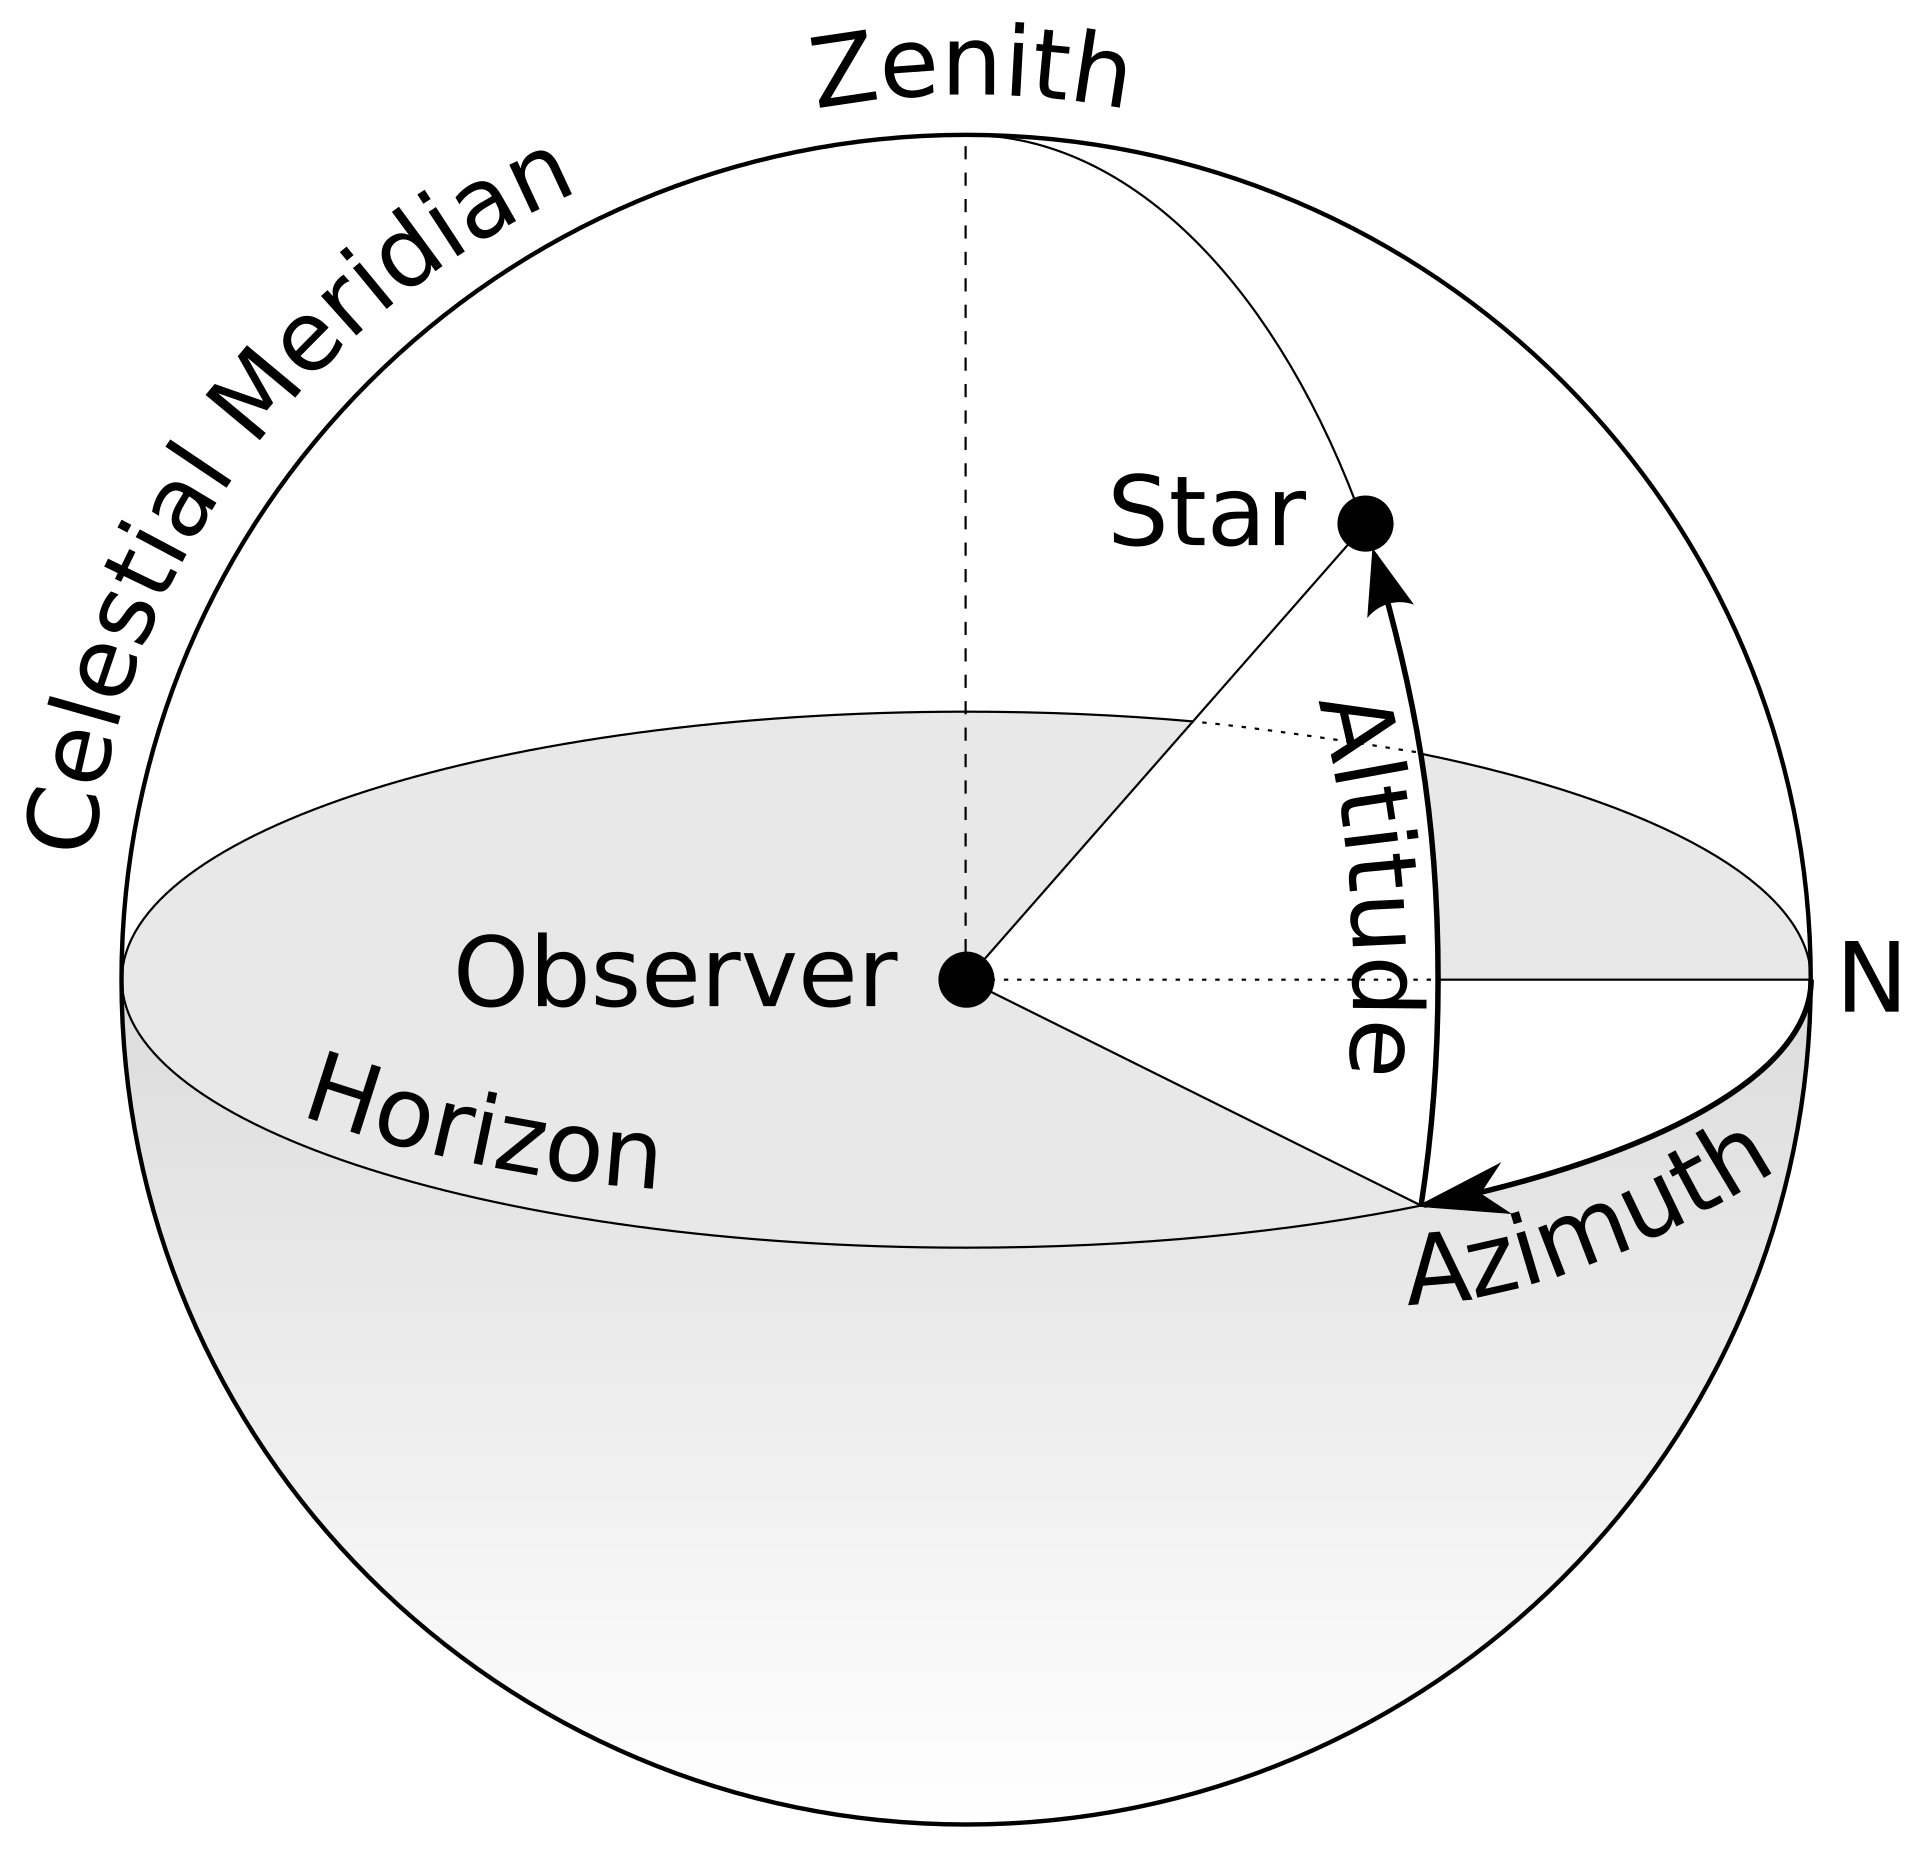
\includegraphics[width=0.98\textwidth]{Astronomy/Azimuth-Altitude_schematic.png}
    \caption{The altitude-azimuth coordinate system used at APEX. Source \cite{altaz_schematic}}
    \label{fig:altaz_coords}
\end{figure}




\section{Radio/(sub)-mm telescope basics}





\begin{figure}[H]
    \centering
    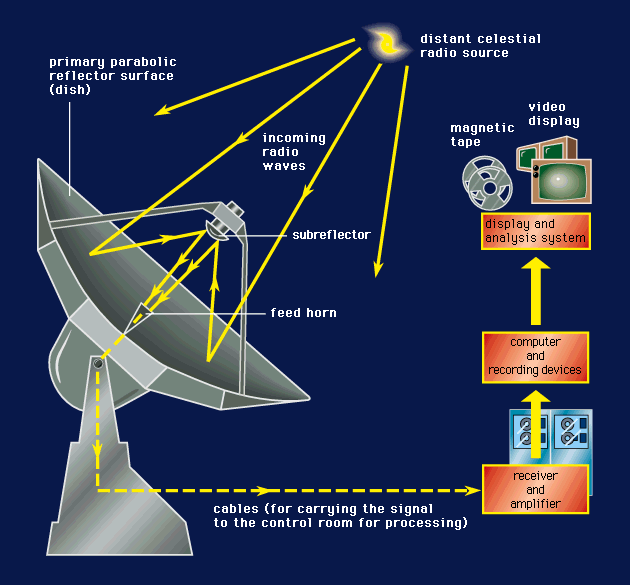
\includegraphics[width=0.98\textwidth]{Astronomy/radio_telescope.png}
    \caption{The main parts of a radio telescope.}
    \label{fig:radio_telescope}
\end{figure}


% \section{Problem description}
% \textcolor{red}{This section have to be fixed completely}
% A telescope makes high precision observations of objects located very far away from Earth.
% Because of this distance, small changes such as the deformation of mirrors due to temperature might impact the precision drastically.\cc{Claudia Cicone: Here you could explain that astronomical objects are observed as they were "projected" in 2D angular coordinates on the sky, and you could talk about astronomical coordinates (see Lecture 5 notes of my course AST2210 for some explanation and references)
% }
% Over time, these deformations have been observed and analyzed, and in order to counter this, a pointing model is made.
% \cc{Claudia Cicone: The need for a pointing model is relevant mainly to sub-mm telescopes that cannot take real-time images of what they are observing, and so the precision of the pointing direction must be known accurately before starting the observations.}
% The pointing model uses measurements from various instruments and is fitted to the observed offsets.
% The model is used for about a month, or until it start performing poorly.
% The variation in measurements are still too big using only this model, so pointing scans have to be made regularly to correct even more.
% A pointing scan is an observation of an object with known location.
% When doing this, the offset on this observation is then added on top of the pointing model.
% These corrections to azimuth and elevations are used for a couple of hours, until a new pointing scan is made.
% \cc{Claudia Cicone: Need to define azimuth and elevation first, see other comment above
% }
% Using this approach, pointing error is reduced to about $4$ arc seconds.\\

% The aim of this thesis is to investigate the possibility of using machine learning to increase the performance of the telescope, by improving pointing accuracy.
% This can be done in multiple ways.

% One possibility is to apply a pointing model on top of the current pointing model using machine learning, such that the average offset is reduced even more.
% Another possibility is investigating the use of machine learning models to aid such that a pointing scan doesn't have to be made as often.
% This will reduce the workload at the telescope. \\

\section{Pointing model}
Since radio/(sub)-mm telescopes observe over an extended time, they need a pointing model to obtain sufficiently accurate pointings.
The flux of the brightest radio sources is also weaker than the atmospheric emission, which means they are invisible in real-time.
Therefore, astronomers must know that the pointing is accurate before making observations.
The pointing model at APEX consists of two parts, one analytical model and additional pointing corrections performed at regular intervals based on recently observed pointing offsets.
These equations can explain the resulting pointing
\begin{align}
    Az &= Az_\text{input} + \Delta Az_\text{analytical model} + \Delta Az_\text{correction} \\ 
    El &= El_\text{input} + \Delta El_\text{analytical model} + \Delta El_\text{correction}
\end{align}
Where the first term is the input coordinates, the second is the adjustment made according to the analytical model,
Furthermore, the last term is the adjustments made according to recent observed pointing offsets.

In the following section, we introduce and explain the adjustments from the analytical model and pointing offsets. 


\subsection{Analytical Model}

Accurately observing pointing offsets without a pointing model can be challenging as the error is typically more significant than the beam size, causing the source to fall outside the beam. At APEX,  they use an optical receiver mounted in the primary mirror to make the initial observations, which allows them to observe the source in real-time.
During this process, the telescope is pointed at various sources with known locations, yielding both input and observed coordinates.

The analytical model at APEX considers various factors that affect pointing, including purely geometrical terms based on the imperfect mounting of telescope components and empirical terms.
The analytical pointing model uses the following terms, dependent on the azimuth $Az$ or elevation $El$, except for a few constant terms.
They determine the coefficients for all the terms using a linear fit based on the observed offsets from a pointing campaign, and the sum of all terms is the adjustment made by the model.

They base most of the terms described in this section on data collected from the optical receiver mounted in the primary mirror.
Then, they refine the terms using observations from different instruments to develop specialized pointing models for each, while most terms remain constant from the optical fit.
The analytical model is crucial in accurately determining the telescope's pointing offsets, essential in obtaining high-quality observational data.

The following descriptions of the terms are taken directly from the tpoint software manual \cite{tpoint_manual}.

\subsubsection{Harmonic terms}
The analytical model has multiple harmonic terms, some geometrical and some empirical.
The tpoint software used to develop the analytical model suggests terms that improve the model's performance on the chosen dataset.
The following terms are the empirical terms for azimuth.
\begin{align}
    \Delta Az =&  c_1 \cdot \sin{Az} + c_2 \cdot \frac{\cos{2Az}}{\cos{El}} + c_3 \cdot \cos{3Az} + c_4 \cdot \sin{2Az} \\
    &+ c_5 \cdot \cos{2Az} + c_6 \cdot \frac{\cos{Az}}{\cos{El}} + c_7 \cdot \frac{\cos{5Az}}{\cos{El}},
\end{align}
and the terms for elevation are

\begin{align}
    \Delta El =&  c_1 \cdot \sin{El} + c_2 \cdot \cos{El}+ c_3 \cdot \cos{2Az} + c_4 \cdot \sin{2Az} \\
    &+ c_5 \cdot \cos{3Az} + c_6 \cdot \sin{3Az} + c_7 \cdot \sin{4Az} + c_8 \cdot \sin{5Az}  
\end{align}


The tpoint software denotes the harmonic terms in the format $Hrfci$. The list below explains the different terms.

\begin{itemize}
    \item $H$: Stands for harmonics
    \item $r$: The resulting variable, either $Az$ or $El$, denoting azimuth and elevation respectively.
    The resulting variable can also be $S$, which means the result is horizontal, or azimuth scaled by a factor $1/\cos{El}$.
    \item $f$: The harmonic function, either $S$ or $C$ denoting \textit{sine} and \textit{cosine}.
    \item $c$: The variable that the funciton $f$ is dependent on, either $Az$ or $El$.
    \item $i$: Integer value in the range $0$-$9$, denoting the frequency of the harmonic.
\end{itemize}

For example, is $\Delta Az = \text{HACA3}\cos{3Az}$ denoted as HACA3 in the tpoint software.

\subsubsection{Az/El non-perpendicularity (NPAE)}
In an altazimuth mount, if the azimuth axis and elevation axis are not exactly at
right angles, horizontal shifts proportional to $\sin{El}$ occur. This effect is zero when pointing at the horizon and increases with elevation proportional to $1/\cos{El}$

\begin{equation}
    \Delta Az \simeq - \text{NPAE } \frac{\sin{El}}{\cos{El}}= - \text{NPAE } \tan{El},
\end{equation}
where NPAE is the horizontal displacement when pointing at Zenith.

\subsubsection{Horizontal displacement of Nasmyth rotator}
In a Nasmyth altazimuth mount, a horizontal displacement between the elevation axis of the mount and the rotation axis of the Nasmyth instrument-rotator produces
and image shift on the sky with a horizontal component
\begin{equation}
    \Delta Az \simeq - \text{NRX},
\end{equation}
and an elevation component
\begin{equation}
    \Delta El \simeq - \text{NRX} \sin{El},
\end{equation}
where NRX is the horizontal displacement.

\subsubsection{Left-right collimation error}
In an altazimuth mount, the collimation error is the non-perpendicularity between the nominated pointing direction and the elevation axis.
It produces a horizontal image shift given by
\begin{equation}\label{eq:pmodel_ca}
    \Delta Az \simeq -\text{CA} / \cos{El}
\end{equation}


\subsubsection{Azimuth and elevation index error}
Index errors are the errors when pointing at origo.

The azimuth index error is 
\begin{equation}
    \Delta Az = -\text{IA},
\end{equation}

and elevation index error is
\begin{equation}\label{eq:pmodel_ie}
    \Delta El = \text{IE}
\end{equation}

\subsubsection{Azimuth axis misalignment} 

In an altazimuth mount, misalignment of the azimuth axis north-south or east-west causes errors.
The errors caused by misalignment in the north-south are given by

\begin{equation}
    \Delta Az \simeq - \text{AN} \sin{Az} \cdot \tan{El},
\end{equation}

and

\begin{equation}
    \Delta El \simeq - \text{AN} \cos{Az},
\end{equation}
where AN is the misalignment alignment in the north-south direction.
The errors given by misalignment in east-west are given by

\begin{equation}
    \Delta Az \simeq - \text{AW} \cos{Az} \tan{El},
\end{equation}

and

\begin{equation}
    \Delta El \simeq \text{AW} \sin{Az},
\end{equation}
where AW is the misalignment alignment in the east-west direction.

\begin{table}[h]
    \centering
    \caption{The terms in the analytical model. \textcolor{red}{Table not complete.} }
    \begin{tabular}{cc}
    \textbf{Azimuth Terms} & \textbf{Elevation Terms} \\
    \hline
    \multicolumn{2}{c}{Optical observations} \\ 
    \cline{1-2}
    \hline
    $\sin{Az}$ & $\sin{El}$ \\
    $\cos{2Az}/\cos{El}$ & $\cos{El}$ \\
    $\cos{3Az}$ & $\cos{2Az}$ \\
    $\sin{2Az}$ & $\sin{2Az}$ \\
    $\cos{2Az}$     & $\cos{3Az}$ \\
    $\cos{Az}/\cos{El}$ & $\sin{3Az}$ \\
    $\cos{5Az}/\cos{El}$ & $\sin{4Az}$ \\
    & $\sin{5Az}$ \\
    \multicolumn{2}{c}{Radio receivers} \\
    \cline{1-2}
    \hline
    $\cos{Az}$ & $\cos{Az}$ \\
    \end{tabular}
\end{table}

\subsection{Pointing corrections} 
The analytical pointing model can only reduce the pointing offsets to about an average of \textcolor{red}{$x$ arcseconds}.
In order to reduce the pointing offsets even further, the astronomers at APEX update the pointing model by pointing at a source with known coordinates.
This operation is called a pointing scan, and by observing the resulting pointing offsets from the known source,
they update the terms CA and IE in the pointing model for azimuth and elevation correction, respectively
They update the terms as follows
\begin{align}
    \text{CA} &= \text{CA} + \delta_{\text{Az}} \label{eq:ca}\\ 
    \text{IE} &= \text{IE} - \delta_{\text{El}},\label{eq:ie},
\end{align}
where $\delta_{\text{Az}}$ and $\delta_{\text{El}}$ are the recently observed pointing offsets in azimuth and elevation, respectively.
The astronomers perform these pointing corrections every couple of hours to ensure the pointing is sufficient during science observations.

Note that we divide the term CA \eqref{eq:pmodel_ca} by cosine elevation, which converts the observed horizontal offset to azimuth.


\section{Research questions and related works}
\begin{itemize}
    \item Reduce poitning offsets with machine learning model
    \item Replace analytical model with machine learning model
    \item reduce the frequency of pointing scans while maintaining pointing accuracy with machine learning model
\end{itemize}

\begin{itemize}
    \item Article about analytical model
    \item ...
\end{itemize}

\section{Database}


\subsection{Raw Data}
The raw data from the pointing scans using the NFLASH230 receiver provides input and actual coordinates.
They obtain the actual coordinates of the sources by combining the input coordinates with the adjustments made by the pointing model,
automatic adjustments based on sensory data, and the observed offset.
Then, they use this raw data to refine the model fit on data obtained from the optical receiver.
Table \ref{tab:raw_datanflash230} is included to provide an example of this data format. 


\begin{table}[h]
    \centering
    \caption{Extract of raw data obtained with NFLASH230. The data file also includes the source, which is irrelevant to this project.}
    \begin{tabular}{ccccc}
         & \multicolumn{2}{c}{Input} & \multicolumn{2}{c}{Observed} \\ 
        \cline{2-3} \cline{4-5}
        Date & Azimuth & Elevation & Azimuth & Elevation \\ 
        \hline
        2022-01-03 14:24:04 & $189.812879$ & $41.0762$ & $190.254779$ & $40.883651$ \\
        2022-01-03 18:59:40 & $50.842145$ & $73.371647$ & $51.269044$ & $73.203243$ \\
        2022-01-03 19:01:49 & $49.555916$ & $73.752182$ & $49.983112$ & $73.583545$ \\
        2022-01-03 19:16:10 & $39.378382$ & $76.076236$ & $39.781084$ & $75.908956$ \\
        2022-01-03 19:18:27 & $113.934309$ & $39.345667$ & $114.391232$ & $39.170168$ \\
        2022-01-22 13:54:31 & $94.04365$ & $18.148405$ & $94.492505$ & $17.981161$ \\
        2022-01-22 14:15:35 & $148.569964$ & $89.044036$ & $147.783271$ & $88.852306$ \\
        2022-01-22 14:18:15 & $215.664924$ & $49.563821$ & $216.104389$ & $49.386438$ \\
    \end{tabular}
    \label{tab:raw_datanflash230}
    \end{table}



\subsection{The Monitor Database}
The monitor database is critical in this project, providing valuable sensory data from within and outside the telescope.
In this section, we will explore the data contained within the monitor database and identify the most relevant variables to our purposes.
We got a copy of the database containing data from 01.01.2022 to 17.09.2022.

\paragraph{Azimuth and Elevation}
The database includes tables for the input azimuth and elevation, labeled COMMANDAZ and COMMANDEL.
These tables contain the raw coordinates before the pointing model has adjusted the pointing.

The database also includes tables for the actual azimuth and elevation, labeled ACTUALAZ and ACTUALEL.
These tables contain the coordinates obtained after applying the pointing model and automatic adjustments based on sensory data.

Finally, the database contains tables for the azimuth and elevation velocity, labeled ACTUALVELOCITYAZ and ACTUALVELOCITYEL.
These tables provide information on the velocity of the telescope during observations.

The frequency of these measurements is $6$ data points per minute.
Figure \ref{subfig:scan_az} show these measurements for the duration of a pointing scan, along with additional data points before and after the scan.


\paragraph{Temperature Measurements}
Multiple instruments located at different locations on the telescope measure the temperature and store the measurements in the database.
The tables that contain these measurements are labeled TEMPERATURE, TEMP1 through TEMP6, TEMP26 through TEMP28, and TILT1T. 
Figure \ref{fig:corr_temp} indicates that many of these measurements are highly correlated.
For example, TEMP1 through TEMP6 show a strong correlation $\geq 0.98$.
Similarly, TEMP26 through TEMP28 and TEMPERATURE are also highly correlated.
The frequencies of some of these measurements are different, and they may all be found in Table \ref{tab:data_frequency}.
Figure \ref{subfig:scan_temp1} and \ref{subfig:scan_tilt1t} show the measurements of TEMP1 and TILT1T respectively
for the duration of a pointing scan and additional data points before and after the scan.


\begin{figure}[H]
    \centering
    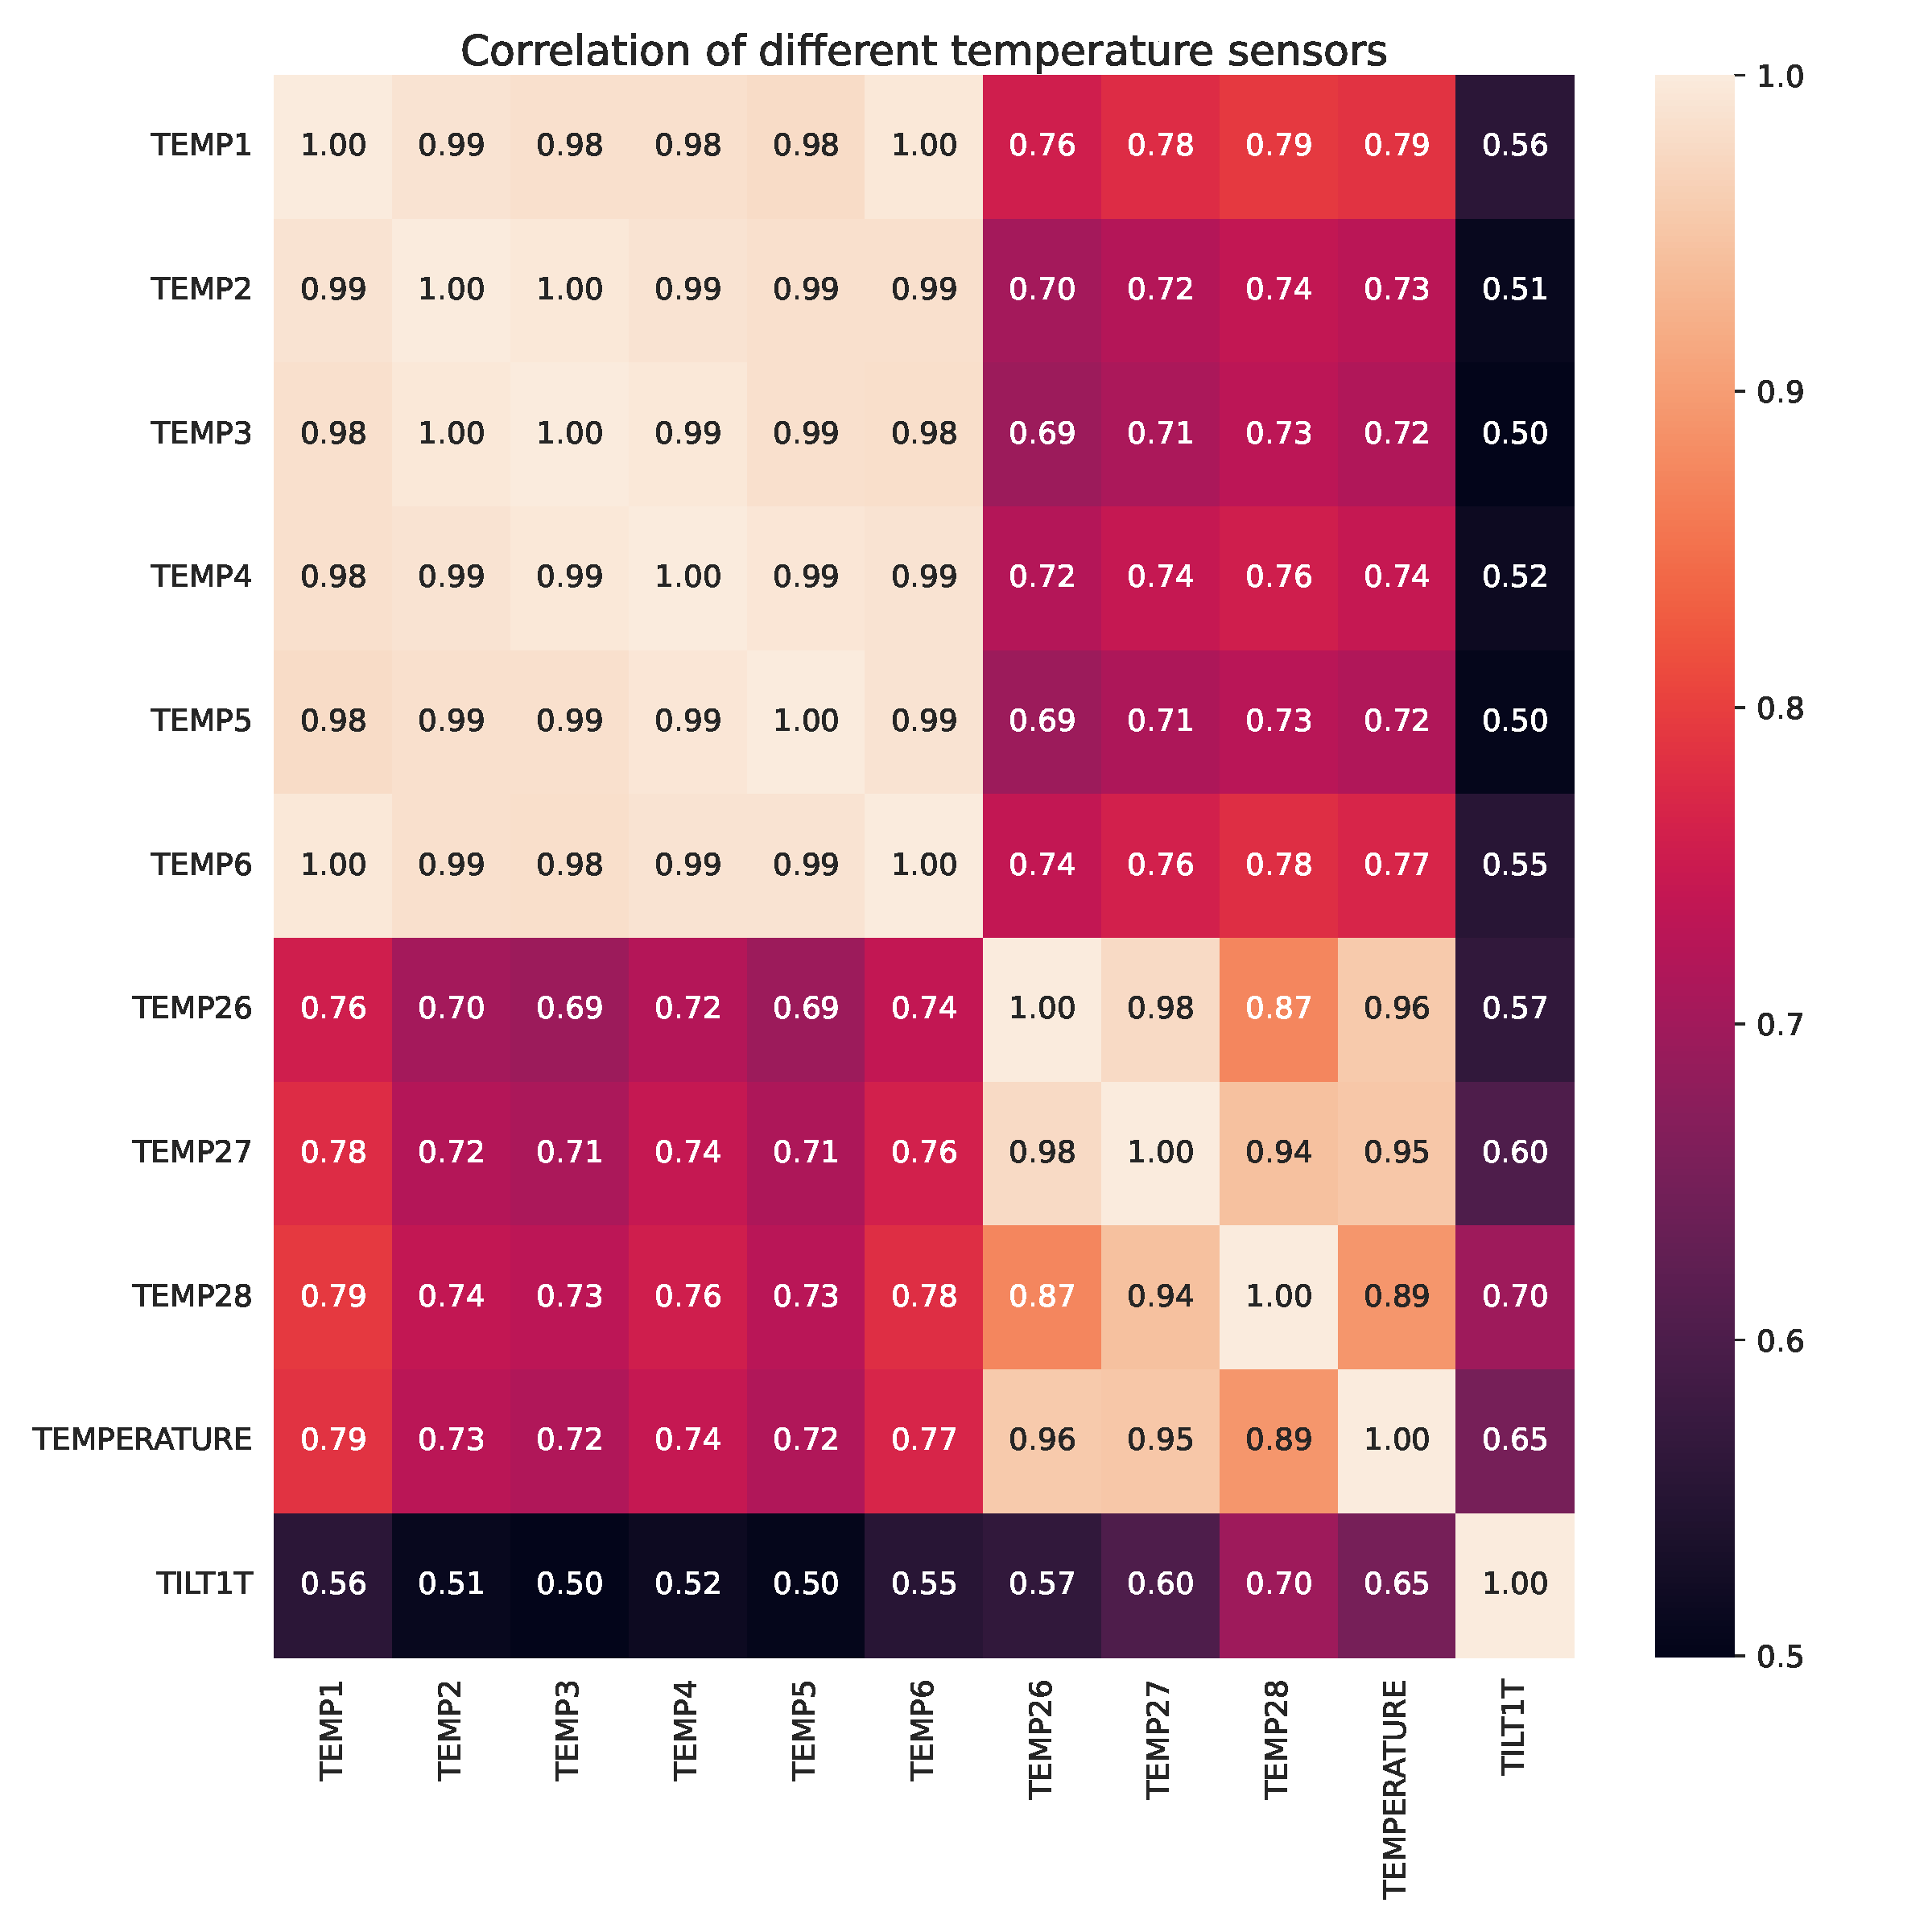
\includegraphics[width=0.98\textwidth]{Correlation/Correlation_temp.pdf}
    \caption{Linear correlation between temperature measures.
    The values are sampled by the median value at each pointing scan.}
    \label{fig:corr_temp}
\end{figure}

\paragraph{Hexapod}
The secondary mirror, also known as the subreflector, is supported by a hexapod.
The hexapod moves in three dimensions and rotates around azimuth and elevation axes.
There are five measures associated with the hexapod: POSITIONX, POSITIONY, POSITIONZ, ROTATIONX, and ROTATIONY.
These measures are essential for positioning the secondary mirror and ensuring accurate pointing. The frequency of these measurements is $6$ data points per minute.

\paragraph{Tiltmeter}
The telescope has two tiltmeters that measure its tilt or inclination to the vertical direction.
One tiltmeter aligns with the telescope's pointing, while the other is orthogonal.
They label these tiltmeters as TILT1X and TILT1Y, respectively, and they take measurements at a frequency of $12$ data points per minute.

\paragraph{Weather data}
The weather station at the telescope provides measurements of various weather parameters, including dew point, humidity, pressure, wind speed, and wind direction.
The instruments take measurements at a frequency of $5$ data points per minute.
The figures \ref{sub@subfig:scan_winddir} and \ref{subfig:scan_windspeed} show wind direction and speed measurements for the time period around a pointing scan.


\paragraph{Disp abs?}

Frequency of $12$ data points per minute.

\paragraph{Automatic adjustments}
Automatic adjustments based on readings from various sensors ensure accurate and stable pointing of the telescope.
These adjustments account for systematic errors previously modeled and are based on measurements from tiltmeters, temperature sensors installed at different locations, and other relevant data sources.
Some system at the telescope automatically makes these adjustments, and the tables in the database that contain information about these adjustments start with DAZ or DEL, denoting adjustments in azimuth and elevation, respectively.
The frequency of this data is $12$ data points per minute.
Table \ref{tab:data_frequency} shows a comprehensive list of these variables.

\paragraph{Data frequency}
The monitor database provides data with varying frequencies, as shown in Table \ref{tab:data_frequency},
which lists the approximate number of data points per minute for each table used in this project.

\begin{table}[H]
    \caption{The frequency in data points per minute of different variables in the monitor database.}
    \centering
    \begin{tabular}{lr}
        \toprule
        Table &  Frequency [datapoints/minute] \\
        \midrule
        ACTUALAZ &                    6 \\
        ACTUALEL &                    6 \\
        ACTUALVELOCITYAZ &                    6 \\
        ACTUALVELOCITYEL &                    6 \\
        COMMANDEL &                    6 \\
        COMMANDAZ &                    6 \\
        TILT1X &                   12 \\
        TILT2Y &                   12 \\
        TILT1T &                   12 \\
        TEMPERATURE &                    5 \\
        TEMP1 &                    6 \\
        TEMP2 &                    6 \\
        TEMP3 &                    6 \\
        TEMP4 &                    6 \\
        TEMP5 &                    6 \\
        TEMP6 &                    6 \\
        TEMP26 &                    2 \\
        TEMP27 &                    2 \\
        TEMP28 &                    2 \\
        DAZ\_TEMP &                   12 \\
        DAZ\_TILT &                   12 \\
        DAZ\_TILTTEMP &                   12 \\
        DAZ\_SPEM &                   12 \\
        DAZ\_DISP &                   12 \\
        DAZ\_TOTAL &                   12 \\
        DEL\_TEMP &                   12 \\
        DEL\_TILT &                   12 \\
        DEL\_TILTTEMP &                   12 \\
        DEL\_SPEM &                   12 \\
        DEL\_DISP &                   12 \\
        DEL\_TOTAL &                   12 \\
        POSITIONX &                    6 \\
        POSITIONY &                    6 \\
        POSITIONZ &                    6 \\
        ROTATIONX &                    6 \\
        ROTATIONY &                    6 \\
        DISP\_ABS1 &                   12 \\
        DISP\_ABS3 &                   12 \\
        DISP\_ABS2 &                   12 \\
        DEWPOINT &                    5 \\
        PRESSURE &                    5 \\
        HUMIDITY &                    5 \\
        WINDSPEED &                    5 \\
        WINDDIRECTION &                    5\\
        \bottomrule
    \end{tabular}
    \label{tab:data_frequency}
\end{table}


\begin{figure}[H]
    \centering
    \begin{subfigure}[t]{0.49\textwidth}
        \centering
        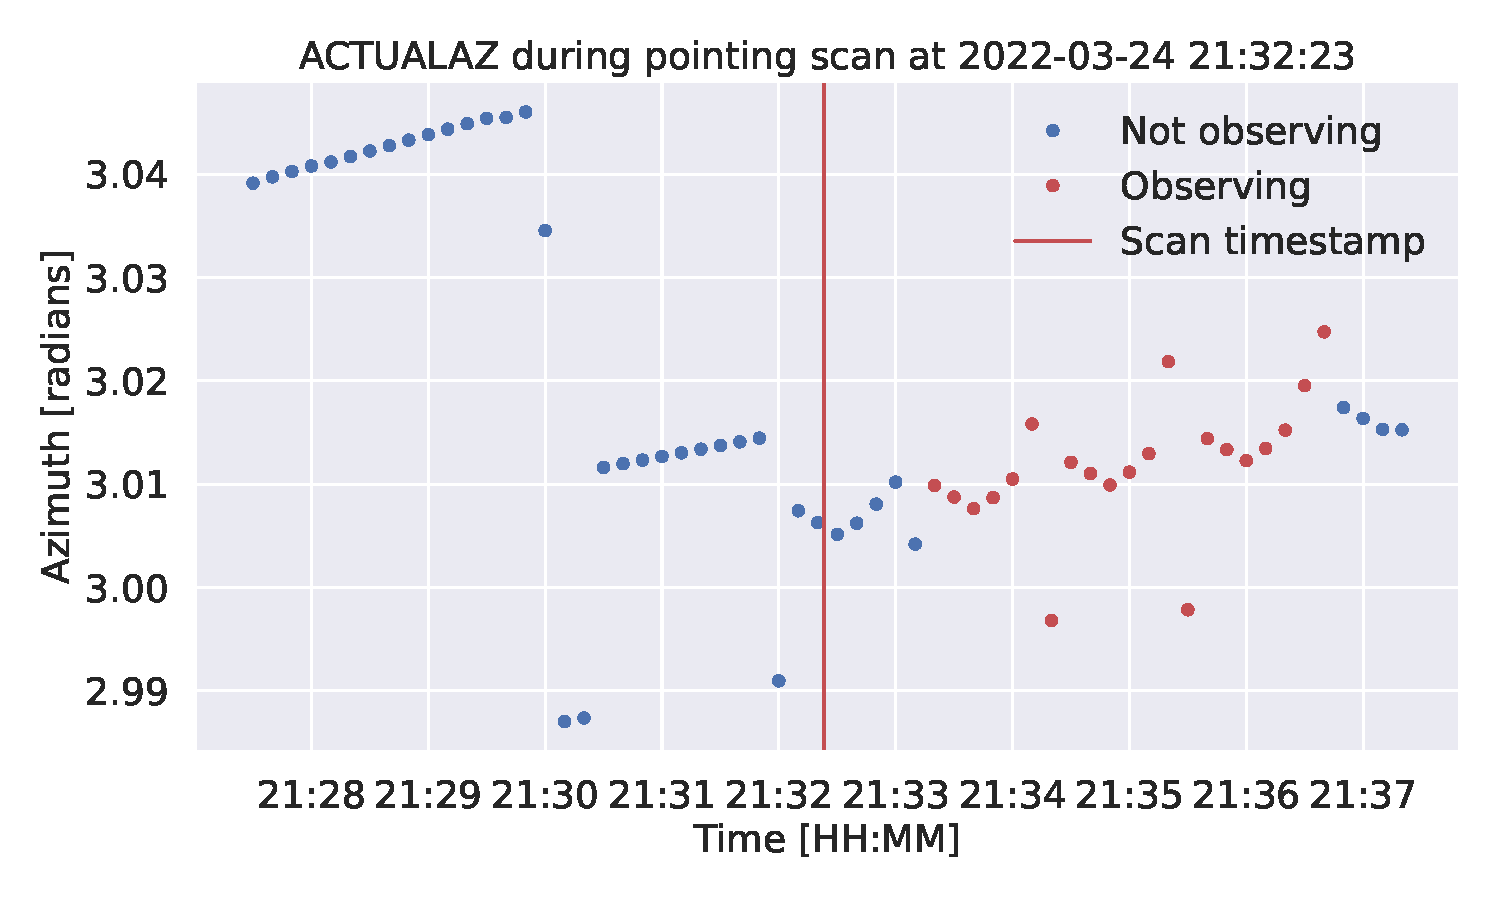
\includegraphics[width=\textwidth]{Feature during scans/scan_ACTUALAZ_335.pdf}
        \caption{Azimuth angle}
        \label{subfig:scan_az}
    \end{subfigure}
    \begin{subfigure}[t]{0.49\textwidth}
       \centering
       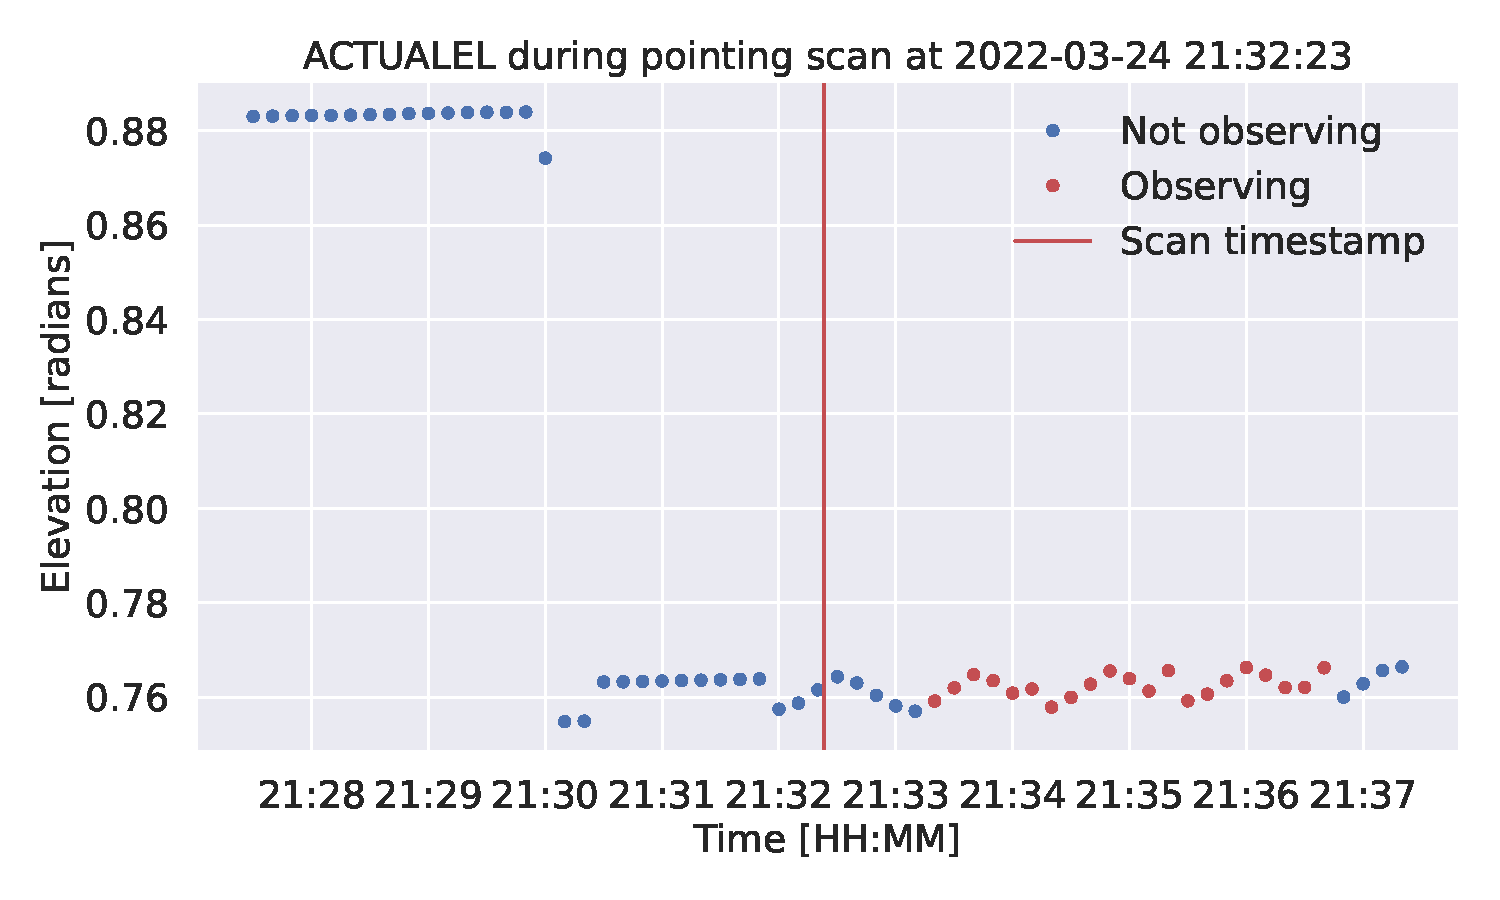
\includegraphics[width=1\textwidth]{Feature during scans/scan_ACTUALEL_335.pdf}
       \caption{Elevation angle.}
       \label{subfig:scan_el}
    \end{subfigure}
    \\~\\
    \begin{subfigure}[t]{0.49\textwidth}
        \centering
        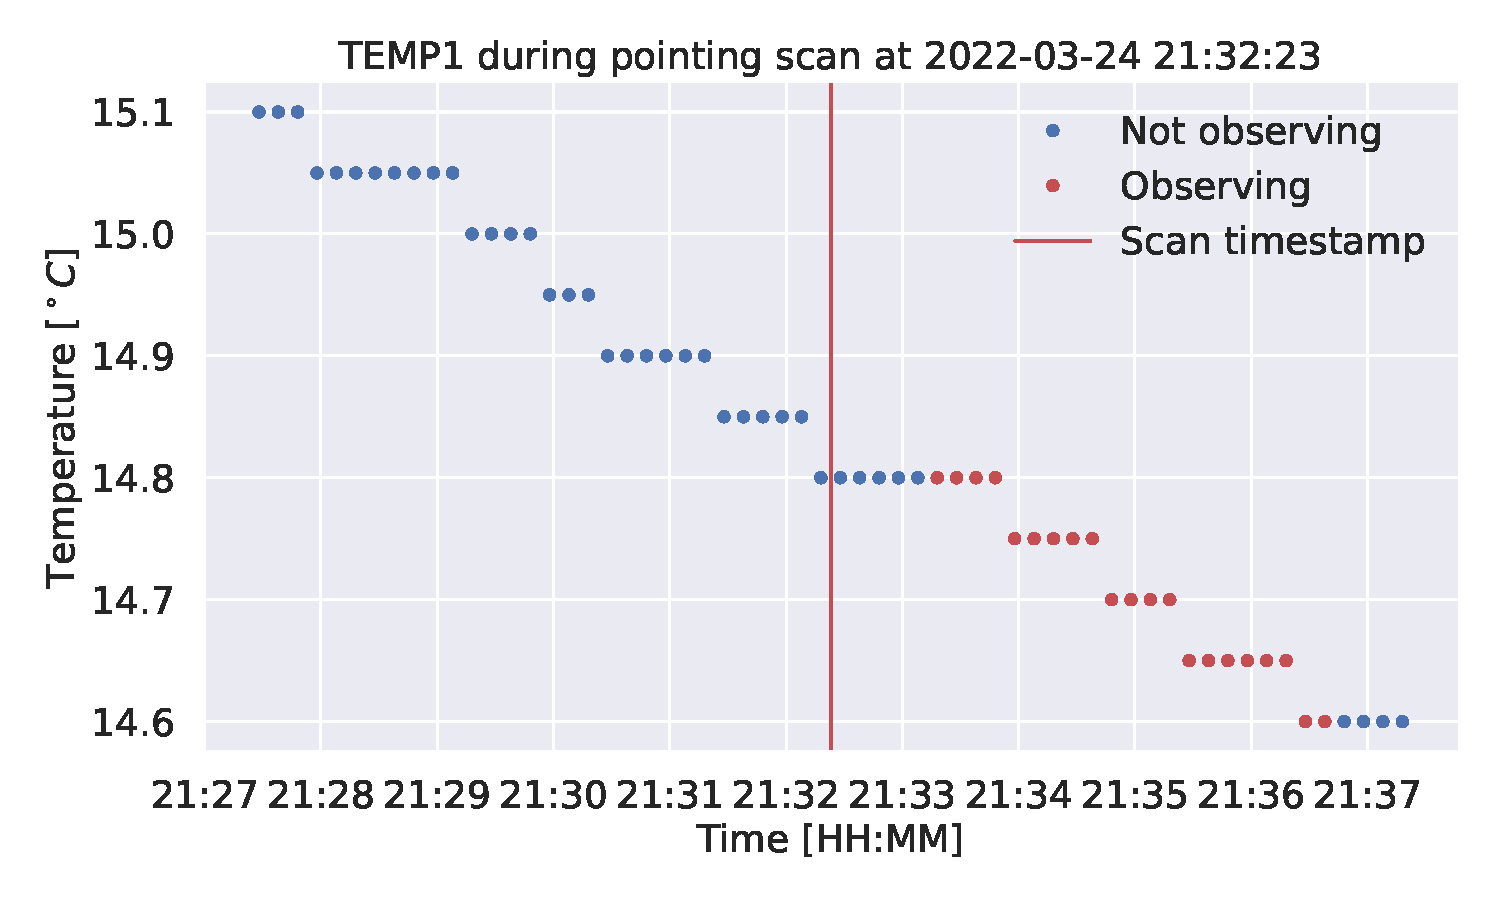
\includegraphics[width=\textwidth]{Feature during scans/scan_TEMP1_335.pdf}
        \caption{Temperature measurements at temperature sensor $1$.}
        \label{subfig:scan_temp1}
    \end{subfigure}
       \begin{subfigure}[t]{0.49\textwidth}
        \centering
        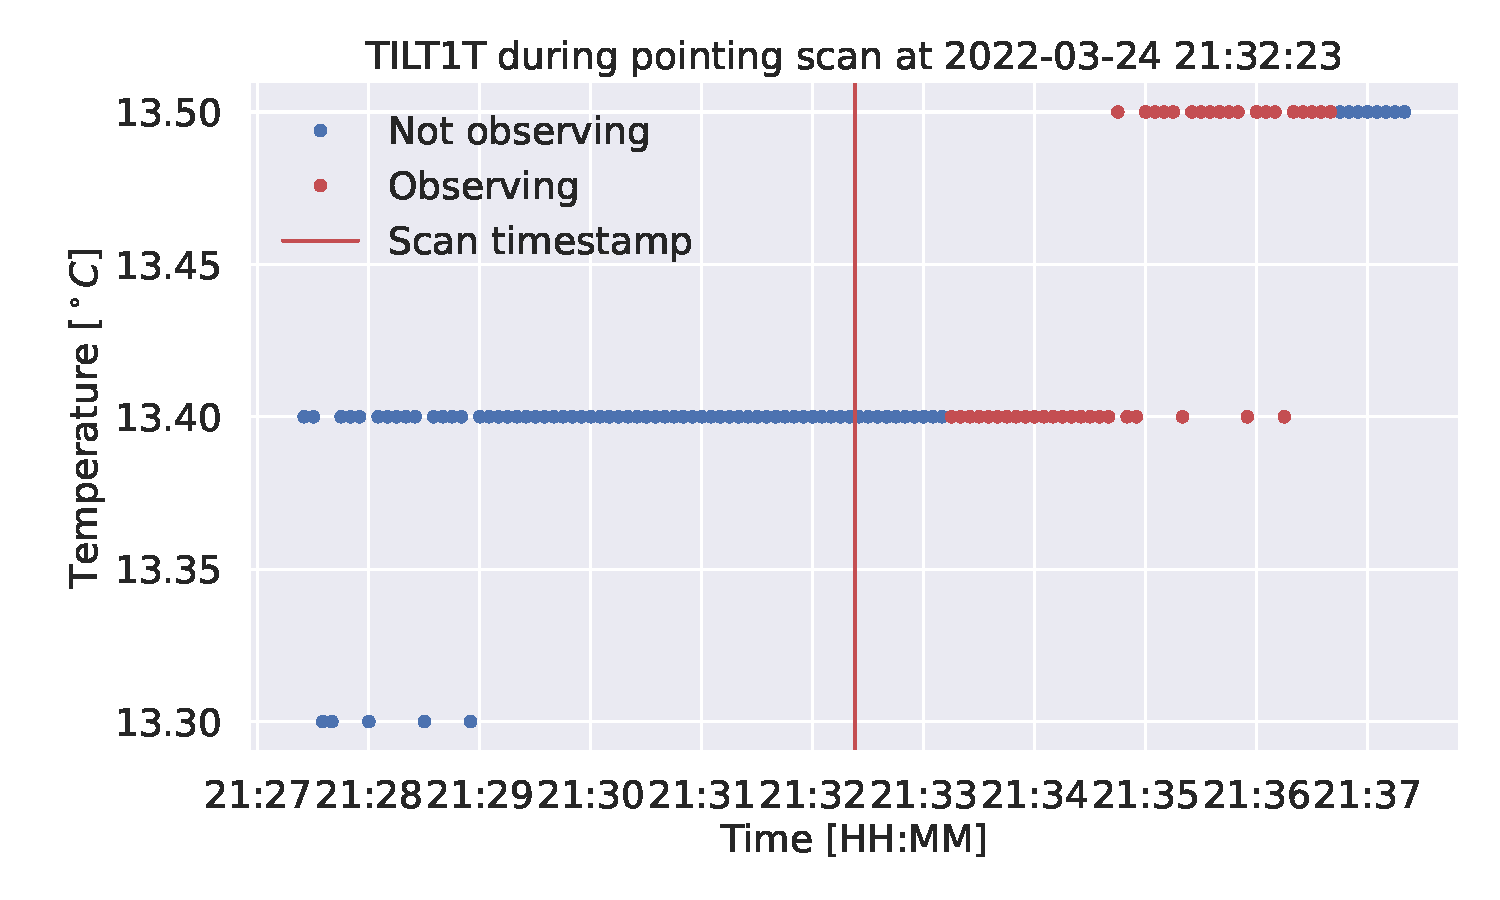
\includegraphics[width=\textwidth]{Feature during scans/scan_TILT1T_335.pdf}
        \caption{Temperature measurements at tiltmeter $1$.}
        \label{subfig:scan_tilt1t}
    \end{subfigure}
    \\~\\
    \begin{subfigure}[t]{0.49\textwidth}
        \centering
        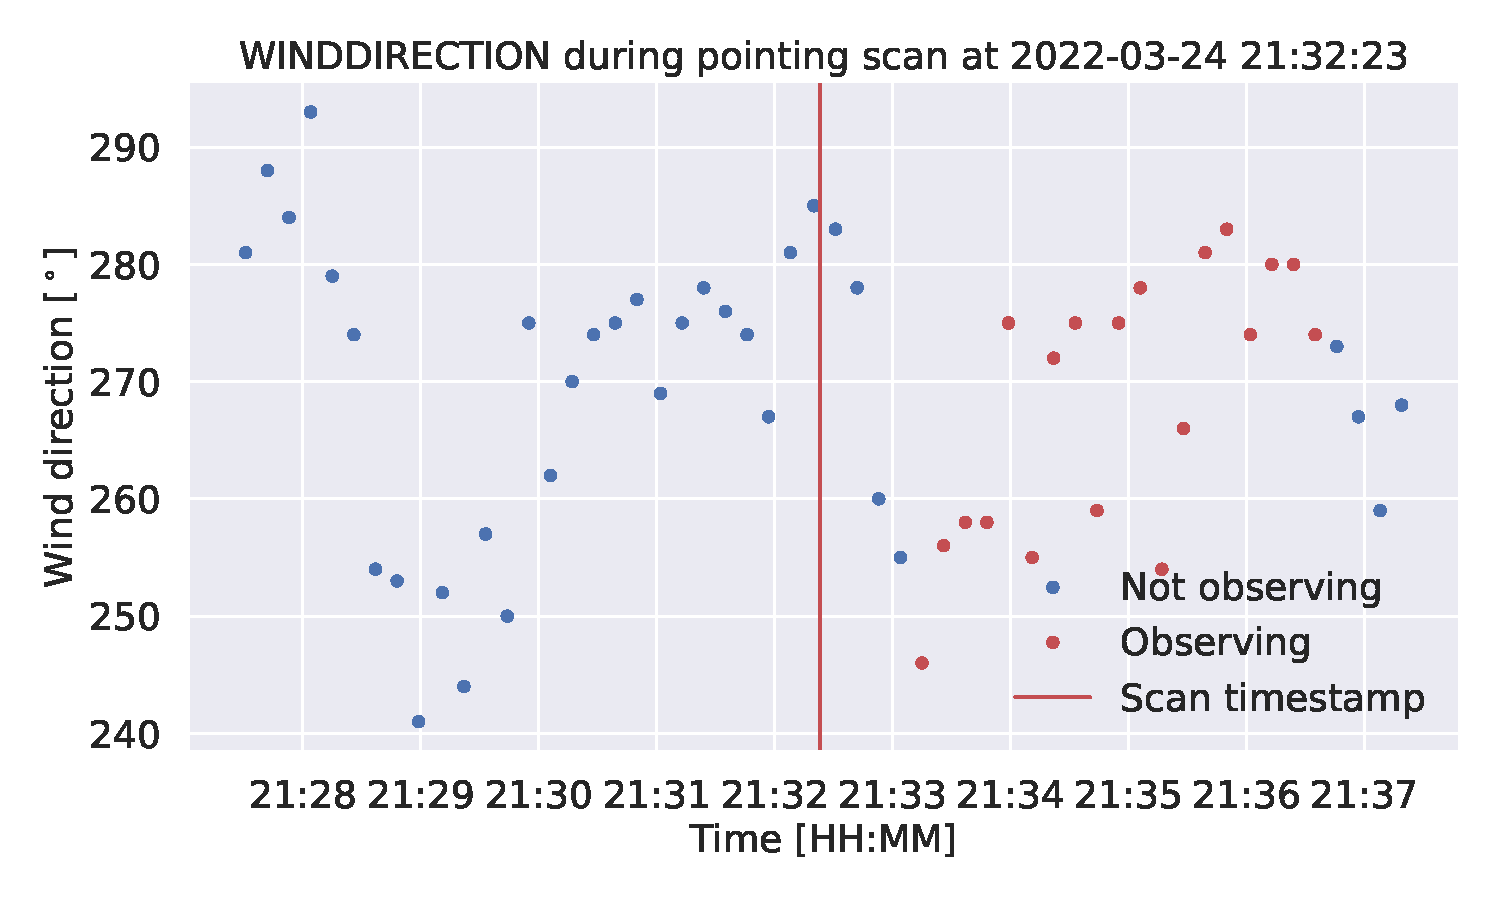
\includegraphics[width=\textwidth]{Feature during scans/scan_WINDDIRECTION_335.pdf}
        \caption{Wind direction data from the weather station, measured in degrees from North, where clockwise is the positive angle direction.}
        \label{subfig:scan_winddir}
    \end{subfigure}
       \begin{subfigure}[t]{0.49\textwidth}
        \centering
        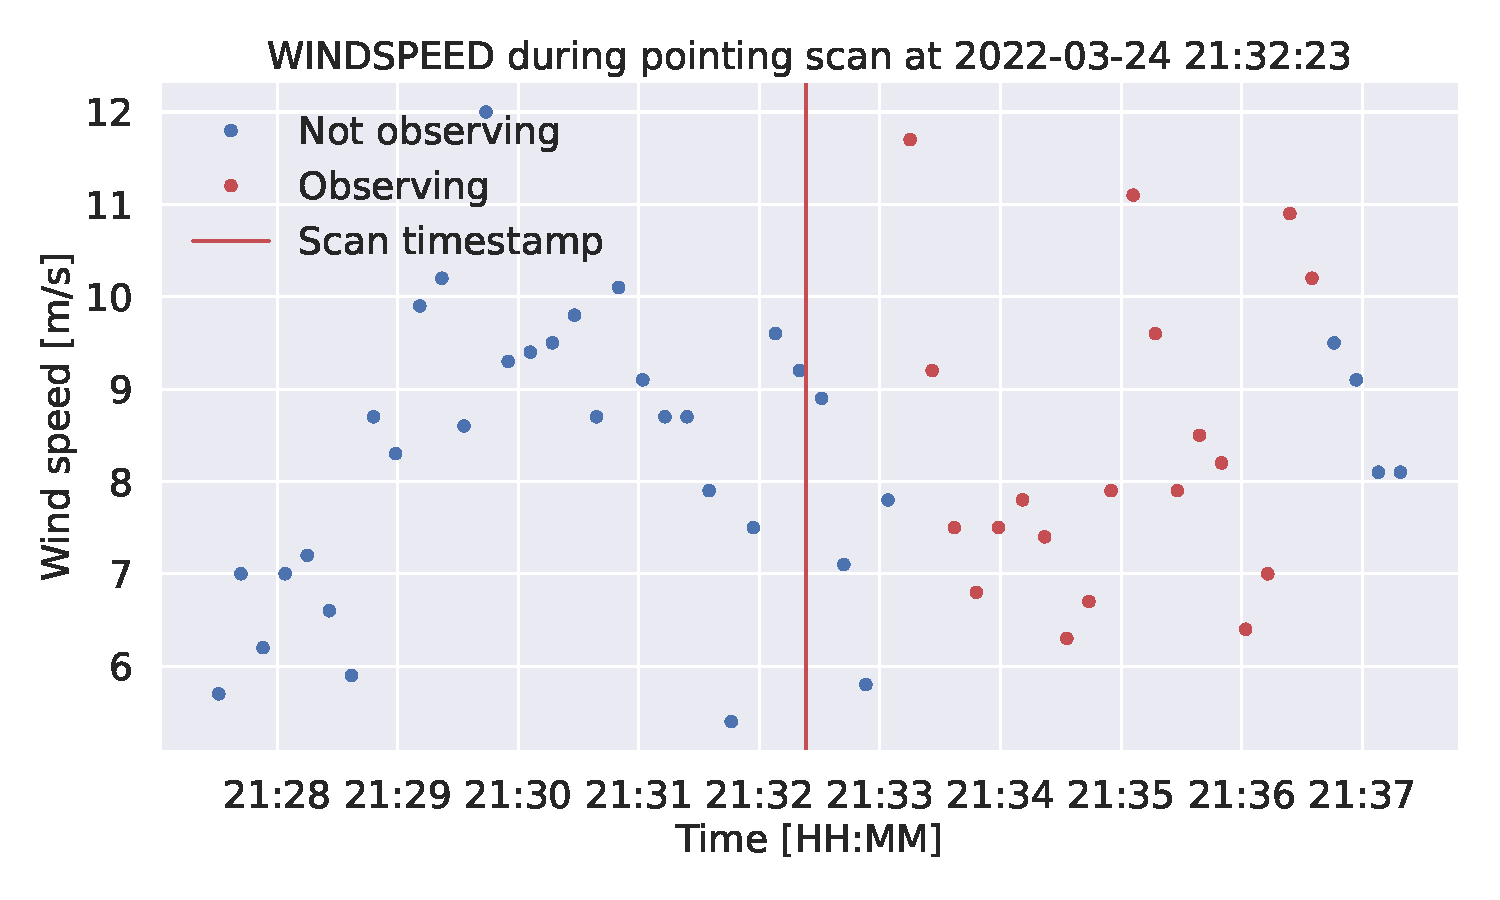
\includegraphics[width=\textwidth]{Feature during scans/scan_WINDSPEED_335.pdf}
        \caption{Wind speed data from the weather station.}
        \label{subfig:scan_windspeed}
    \end{subfigure}
     \caption{Scatter plots that show different sensory data from before, during, and after a pointing scan. The red line denotes the timestamp for a scan in the pointing scan database.
     The red dots indicate when the telescope is observing, while the blue dots indicate when the telescope is idle or preparing to observe.}
     \label{fig:features_during_scans}
\end{figure}


\subsection{Pointing scan data}
During a pointing scan, the telescope observes a source with a known location to obtain a pointing offset.
The observers use this offset to recalibrate the pointing model. There are two types of pointing scans: Line-pointings and continuum scans.
Figure \ref{fig:features_during_scans} shows the information in the monitor database from a pointing scan.

\paragraph{Line-pointing}
A line-pointing involves pointing at an extended source. 
The telescope then makes ten scans, recording the flux intensity from the source, five vertically and five horizontally,
around the center of the pointing, as shown in figure \ref{fig:line_pointings}.
The upper panel shows a high-quality pointing scan, and the lower panel shows a noisy, low-quality pointing scan.
The cross-plot on the right side shows the line spectrum for each observation (center plus eight offset observations).

The integrals of the flux recorded from the source are plotted as blue dots on the left-hand side of the panel.
A Gaussian is fitted to these points, and the table shows the resulting amplitude, full width at half maximum (FWHM), and offsets.

\begin{figure}[H]
    \centering
     \begin{subfigure}[b]{0.75\textwidth}
         \centering
         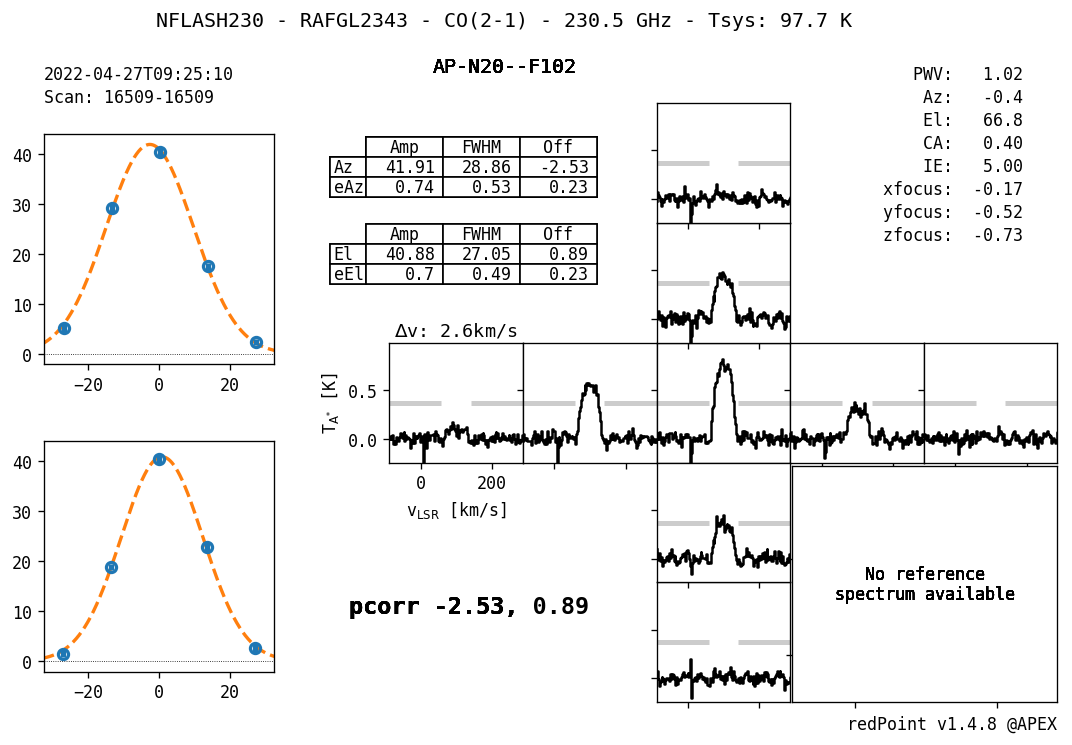
\includegraphics[width=\textwidth]{Pointing Scans/good_line.png}
         \caption{Line-pointing with little noise and a good Gaussian fit.}
         \label{subfig:good_line}
     \end{subfigure}
    \\
     \begin{subfigure}[b]{0.75\textwidth}
         \centering
         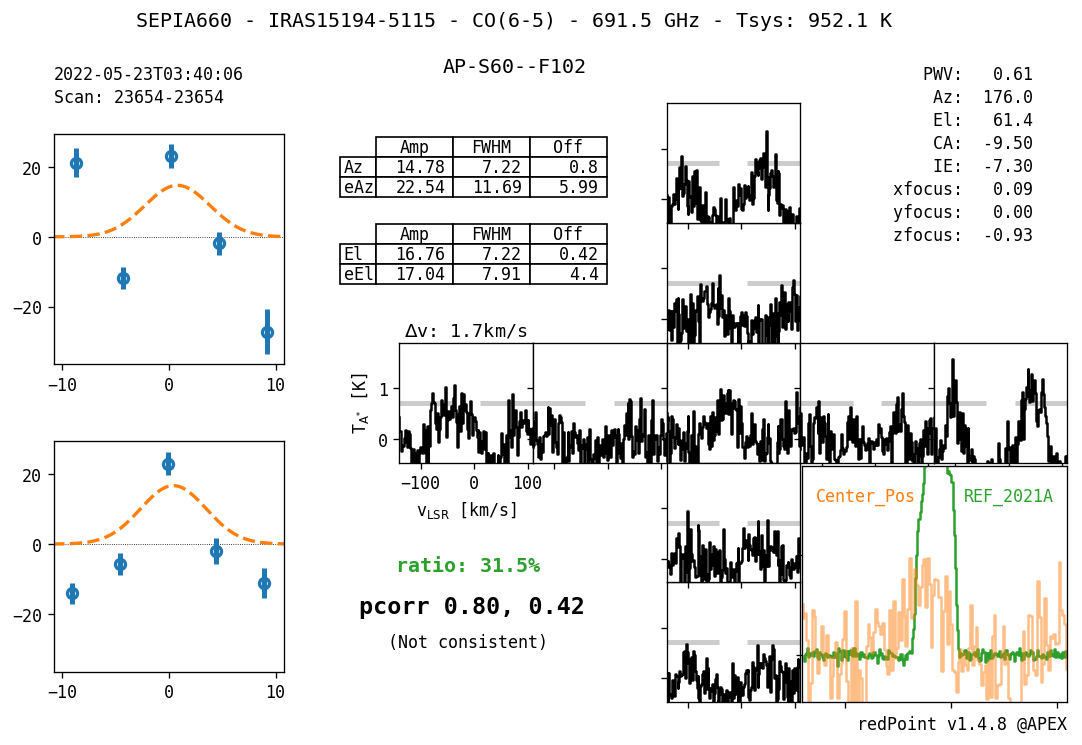
\includegraphics[width=\textwidth]{Pointing Scans/bad_line.png}
         \caption{Noisy line-pointing with bad Gaussian fit.}
         \label{subfig:bad_line}
     \end{subfigure}
    \caption{The two figures show line-pointing scans. a) is good and clean, and b) is noisy and unreliable. A Gaussian is fit both for the azimuth and elevation pointing.
    The table shows the amplitude, full width at half maximum (FWHM), offset, and the uncertainty of these measures, for azimuth and elevation.
    The figures also show the correction applied during the pointing ($ca$ and $ie$), along with other metrics.}
    \label{fig:line_pointings}
\end{figure}

\paragraph{Continuum Scan}
Not all sources have emission lines; for these sources, the telescope performs a continuum scan instead. In this case, a source is continuously scanned in azimuth and elevation while recording the flux intensity.
A Gaussian curve is fitted to the recorded flux intensity to determine the offsets, amplitude, and full width at half maximum (FWHM).
Figure \ref{fig:continueous_pointings} show examples of continuum scans and the corresponding Gaussian fits.

\begin{figure}[H]
    \centering
     \begin{subfigure}[b]{0.75\textwidth}
         \centering
         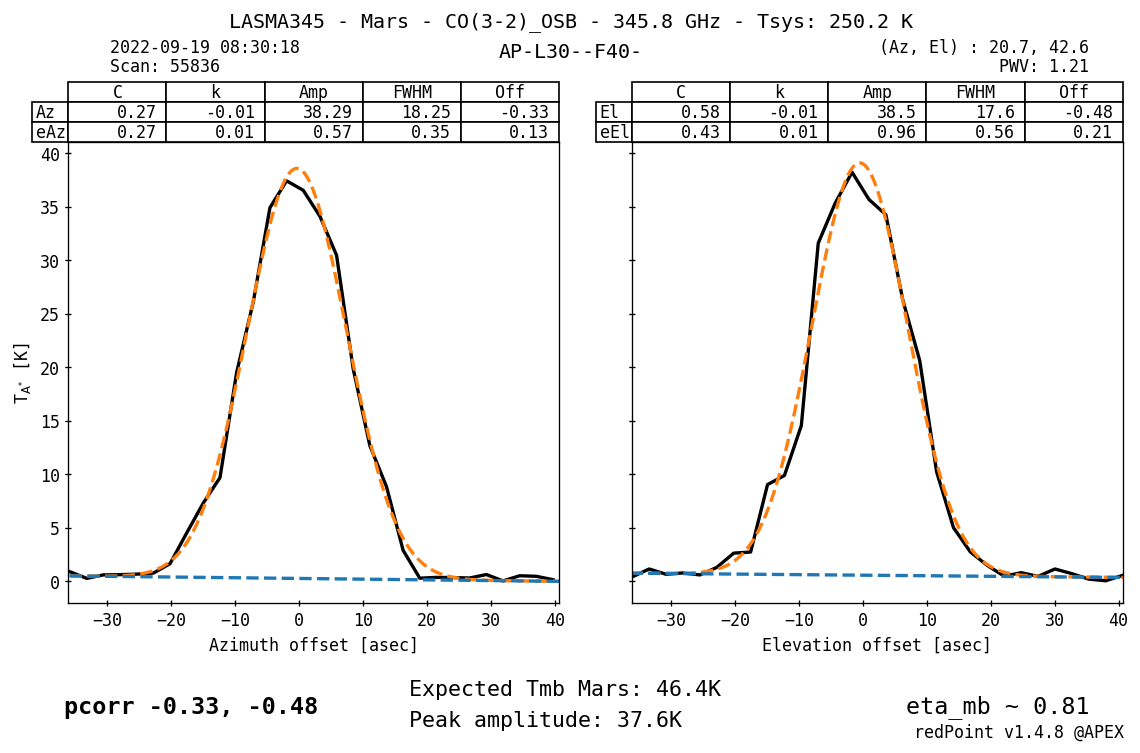
\includegraphics[width=\textwidth]{Pointing Scans/good_continuous.png}
         \caption{Line-pointing with little noise and a good Gaussian fit.}
         \label{subfig:good_continuous}
     \end{subfigure}
    \\
     \begin{subfigure}[b]{0.75\textwidth}
         \centering
         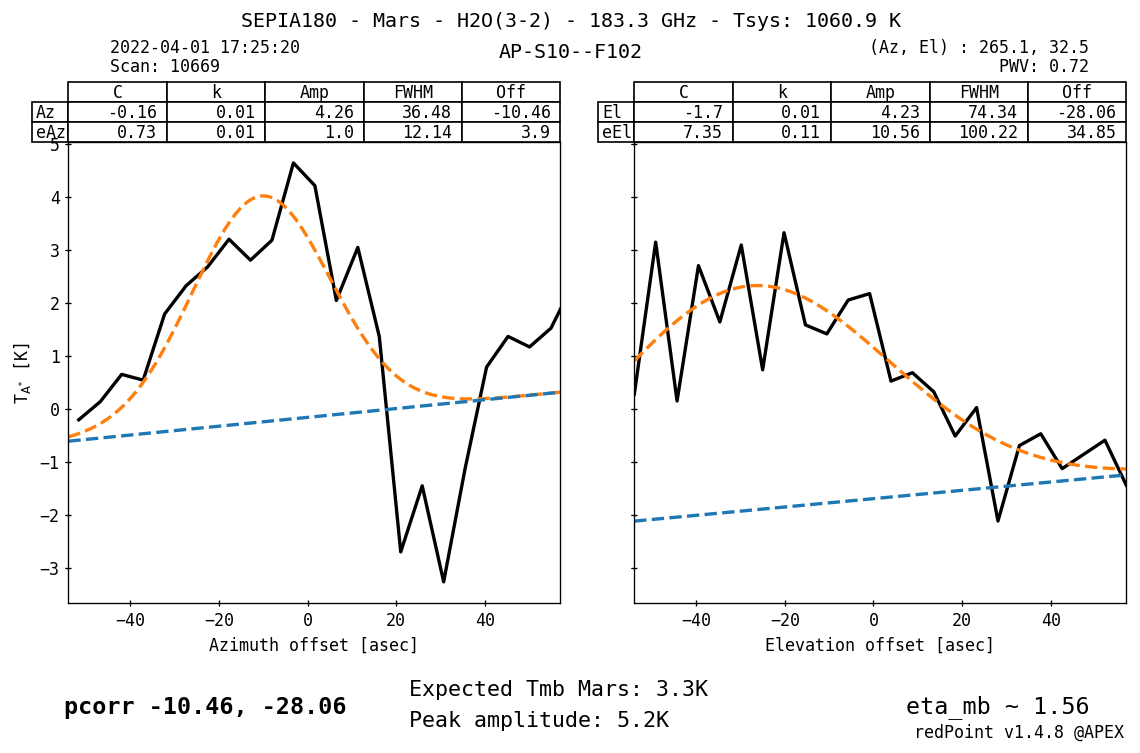
\includegraphics[width=\textwidth]{Pointing Scans/bad_continuous.png}
         \caption{Noisy line-pointing with bad Gaussian fit.}
         \label{subfig:bad_continuous}
     \end{subfigure}
    \caption{The two panels show continuum pointing scans. a) is good and clean, and b) is noisy and unreliable. A Gaussian is fit both for the azimuth and elevation pointing. The amplitude, full width at half maximum, offset, and the uncertainty of these measures are shown for both of the fits.}
    \label{fig:continueous_pointings}
\end{figure}



\paragraph{Pointing scan timestamp} 
In the main database, each pointing scan has a timestamp in the format YYYY-MM-DD HH:MM:SS, with a one-second resolution. This timestamp does not reflect the actual start of a pointing scan. Also, there is not information in the database itself that indicates whether the telescope is observing, but this information can be extracted from some dump files from the tiltmeter, which includes a flag indicating whether the telescope is idle, preparing to observe, or observing. Combining this flag with the timestamps, we can obtain the accurate start and end time of a pointing scan. However, these tiltmeter dump files are only available for some time periods.

\begin{itemize}
    \item Plots with scan times distribution
    \item proportion of scans we have the accurate time for
    \item What we did for hte other scans
    \item mention some deviation
\end{itemize}

\paragraph{Instruments}
The observing instruments on the telescope operate at various frequencies.
Table \ref{tab:instrument_usage} provides information on the frequency range covered by each instrument,
along with the number of scans performed using each instrument throughout the year 2022.\\

The broad range of frequencies at which astronomical phenomena emit electromagnetic radiation requires observation across a wide range of frequencies to study these phenomena comprehensively.
APEX's \href{https://www.eso.org/sci/facilities/apex/cfp/cfp110/instrument_summary.html.html}{website} provides a complete list of instruments along with their descriptions.
\begin{table}[H]
    \centering
    \caption{The number of times each instrument was used for a pointing scan in $2022$. There are $8847$ scans in total.}
    \begin{tabular}{lcr}
        \toprule
        Instrument & Frequency band [GHz] &\# of scans \\
        \midrule
        NFLASH230 & $200$-$270$ &3197 \\
        LASMA345  & $268$-$375$ &1861 \\
        NFLASH460 & $385$-$500$ &1394 \\
        SEPIA660  & $578$-$738$ & 856 \\
        SEPIA345  & $272$-$376$ & 818 \\
        SEPIA180  & $159$-$211$ & 359 \\
        HOLO      & - & 225 \\
        ZEUS2     & - & 103 \\
        CHAMP690  & - &  34 \\
        \bottomrule
        \end{tabular}
        \label{tab:instrument_usage}
\end{table}



\subsection{Tiltmeter dump files}
The tiltmeter dump files are a small part of the database and are only used to analyze when pointing scans start and end.
There are 280 of these files, and all have filenames in the format "Tiltmeter\_YYYY-MM-DD.dump," which indicates the data's date.
These files contain seven columns: datetime, azimuth, elevation, tilt1x, tilt1y, tilt1t, and the scan flag.
For our purpose, only the datetime and scan flags provide useful information.
Table \ref{tab:tiltmeter_example} shows an extract of the datetime and scan flag columns from one of the tiltmeter dumps.


\begin{table}[H]
    \centering
    \caption{Extract from a tiltmeter dump file.}
    \begin{tabular}{cc}
        \toprule
        Datetime & Scan flag \\
        \midrule
        2022-11-13T02:23:37 & IDLE \\
        2022-11-13T02:23:38 & IDLE \\
        2022-11-13T02:23:39 & PREPARING \\
        2022-11-13T02:23:40 & PREPARING \\
        $\vdots$ & $\vdots$ \\ 
        2022-11-13T02:23:52 & PREPARING \\
        2022-11-13T02:23:53 & PREPARING \\
        2022-11-13T02:23:55 & OBSERVING \\
        2022-11-13T02:23:56 & OBSERVING \\
        2022-11-13T02:23:57 & OBSERVING \\
        \bottomrule
    \end{tabular}
    \label{tab:tiltmeter_example}
\end{table}